\documentclass[sans,mathserif,aspectratio=169, 10pt]{beamer}

\usepackage{booktabs}
\usepackage[spanish, mexico]{babel}
\selectlanguage{spanish}
\decimalpoint
\usepackage[utf8]{inputenc}
\usepackage{fourier}
\newcommand{\quotes}[1]{``#1''}
\usepackage{epstopdf}
\usepackage{mathtools}
\DeclarePairedDelimiter{\ceil}{\lceil}{\rceil}
\usepackage{commath}
\usepackage{amsmath,tabularx}
\usepackage{listings}
\usepackage{xcolor}
\usepackage[edges]{forest}
\graphicspath{{Images/}}
\usepackage[mathscr]{euscript}
\newcommand{\overbar}[1]{\mkern 1.5mu\overline{\mkern-1.5mu#1\mkern-1.5mu}\mkern 1.5mu}
\newcommand*\mean[1]{\overbar{#1}}
\usepackage{relsize}

\newcommand\Fontvi{\fontsize{9}{7.2}\selectfont}
\definecolor{foldercolor}{RGB}{124,166,198}

%Tikz stuff
\usepackage{tikz}
\usetikzlibrary{trees}
\usetikzlibrary{shapes,arrows,positioning}
\usepackage{forest}

\colorlet{punct}{red!60!black}
\definecolor{background}{HTML}{EEEEEE}
\definecolor{delim}{RGB}{20,105,176}
\colorlet{numb}{magenta!60!black}

\lstdefinelanguage{json}{
    basicstyle=\normalfont\ttfamily\tiny,
    columns=flexible,
    keepspaces=true,
    frame=lines,
    backgroundcolor=\color{background}
}

%Forest Set
\tikzset{
    invisible/.style={opacity=0,text opacity=0},
    visible on/.style={alt=#1{}{invisible}},
    alt/.code args={<#1>#2#3}{%
      \alt<#1>{\pgfkeysalso{#2}}{\pgfkeysalso{#3}} % \pgfkeysalso doesn't change the path
    },
}
\forestset{
  visible on/.style={
    for tree={
      /tikz/visible on={#1},
      edge={/tikz/visible on={#1}}}}}

\mode<presentation>

%Colors
\definecolor{steel}{RGB}{52,102,136}
\definecolor{moss}{RGB}{139,187,159}
\definecolor{burnt}{RGB}{187,102,65}
\definecolor{sandy}{RGB}{186, 168, 111}
\definecolor{RoyalBlue}{RGB}{0,35,102}
\definecolor{cream}{RGB}{254, 246, 235}
\definecolor{slate}{RGB}{82, 85, 100}
\definecolor{fall}{RGB}{194, 91, 86} % frame color
\definecolor{light}{RGB}{150, 192, 206}

% Tikz Image Extras
%Colors
\definecolor{buttercup}{RGB}{245,204,93}
\definecolor{calypso}{RGB}{51,102,136}
\definecolor{casper}{RGB}{170,196,209}
\definecolor{beige}{RGB}{254,250,225}
\definecolor{grenadier}{RGB}{193,49,0}
\definecolor{chiffon}{RGB}{255,251,208}
\definecolor{tawny}{RGB}{204,102,0}
\definecolor{danube}{RGB}{102,153,204}
\definecolor{rich}{RGB}{162,95,8}
\definecolor{york}{RGB}{122,186,122}
\definecolor{royals}{RGB}{18,55,143}
\definecolor{powder}{RGB}{96,164,223}
\definecolor{gold}{RGB}{247,204,019}
\definecolor{columbia}{RGB}{117,178,221}
\definecolor{crater}{RGB}{179,53,18}

\definecolor{grey}{RGB}{168,168,168}
\definecolor{chair}{RGB}{179,133,65}
\definecolor{navy}{RGB}{9,40,105}

\newcommand\blfootnote[1]{%
  \begingroup
  \renewcommand\thefootnote{}\footnote{#1}%
  \addtocounter{footnote}{-1}%
  \endgroup
}

%Tikz Styles
\tikzstyle{mybox} = [draw=grenadier, fill=chiffon, very thick, dashed, rectangle, rounded corners, 
    inner sep=10pt]
\tikzstyle{title} = [fill=grenadier, text=white]
\tikzstyle{program} = [rectangle, rounded corners, fill=grenadier!75, text centered, text width=5em,inner sep=10pt]
\tikzstyle{external} = [rectangle, rounded corners, fill=columbia, text centered, text width=5em,inner sep=10pt]
\tikzstyle{tool} = [rectangle, rounded corners, fill=york, text centered, text width=7em,inner sep=10pt]
\tikzstyle{input} = [rectangle, rounded corners, fill=danube, text centered, text width=5em]
\tikzstyle{proposal} = [rectangle, very thick, dashed, fill=grenadier!95, text centered]
\tikzstyle{line} = [draw, -latex']
    

%Structure
\usefonttheme{professionalfonts}
\hypersetup{colorlinks,linkcolor=fall!80,urlcolor=fall!80}
\setbeamercolor{local structure}{fg=fall}
\setbeamercolor{background canvas}{bg=cream}
\setbeamercolor{frametitle}{bg=fall,fg=cream}
\setbeamercolor{title}{fg=steel!115}
\setbeamercolor{author}{fg=fall}

\defbeamertemplate*{title page}{customized}[1][]
{\centering
  \usebeamerfont{subtitle}\usebeamercolor[fg]{subtitle}\insertsubtitle\par
  \usebeamerfont{title}\usebeamercolor[fg]{title}{\bfseries\inserttitle}\par
  \vfill
  \usebeamerfont{author}\usebeamercolor[fg]{author}\insertauthor\par
  \vfill
  \usebeamerfont{institute}\insertinstitute\par
  \usebeamerfont{date}\insertdate\par
  \usebeamercolor[fg]{titlegraphic}\inserttitlegraphic
}

% Progressbar
\usepackage{tikz}
\usetikzlibrary{calc}

\makeatletter
\def\progressbar@progressbar{} % the progress bar
\newcount\progressbar@tmpcounta% auxiliary counter
\newcount\progressbar@tmpcountb% auxiliary counter
\newdimen\progressbar@pbht %progressbar height
\newdimen\progressbar@pbwd %progressbar width
\newdimen\progressbar@tmpdim % auxiliary dimension

\progressbar@pbwd=\paperwidth
\progressbar@pbht=2pt

\def\progressbar@progressbar{%

\progressbar@tmpcounta=\insertframenumber
\progressbar@tmpcountb=\inserttotalframenumber
\progressbar@tmpdim=\progressbar@pbwd
\multiply\progressbar@tmpdim by \progressbar@tmpcounta
\divide\progressbar@tmpdim by \progressbar@tmpcountb

  \begin{tikzpicture}[very thin]

  \shade[draw=steel!115,top color=steel,bottom color=steel,middle color=steel!115] %
    (0pt, 0pt) rectangle ++ (\progressbar@tmpdim, \progressbar@pbht);

  \end{tikzpicture}%
 }

\addtobeamertemplate{frametitle}{}
{%
  \vspace*{-16pt}
  \begin{beamercolorbox}[wd=\paperwidth,ht=1pt,dp=1pt]{}%
    \progressbar@progressbar%
  \end{beamercolorbox}%
}%
\makeatother

%Title
\title{Proposed Verification Methodology for Resonance Calculations in Gemma}
\subtitle{Thesis Project Research Topics}
\author[Guillermo Ibarra]{Guillermo Ibarra Reyes\\{\small Supervised by: Dr Gustavo Alonso Vargas}}
\date{ESFM Nuclear Engineering Research Seminar, December 8th, 2020}

\definecolor{keywords}{RGB}{255,0,90}
\definecolor{comments}{RGB}{0,0,113}
\definecolor{red}{RGB}{160,0,0}
\definecolor{green}{RGB}{0,150,0}

\setbeamercovered{transparent}
\setbeamercovered{%
  again covered={\opaqueness<1->{40}}}
\beamertemplatenavigationsymbolsempty

\begin{document}

%slide
\begin{frame}
\titlepage
\end{frame}

\begin{frame}
\centering
\fcolorbox{fall}{white}{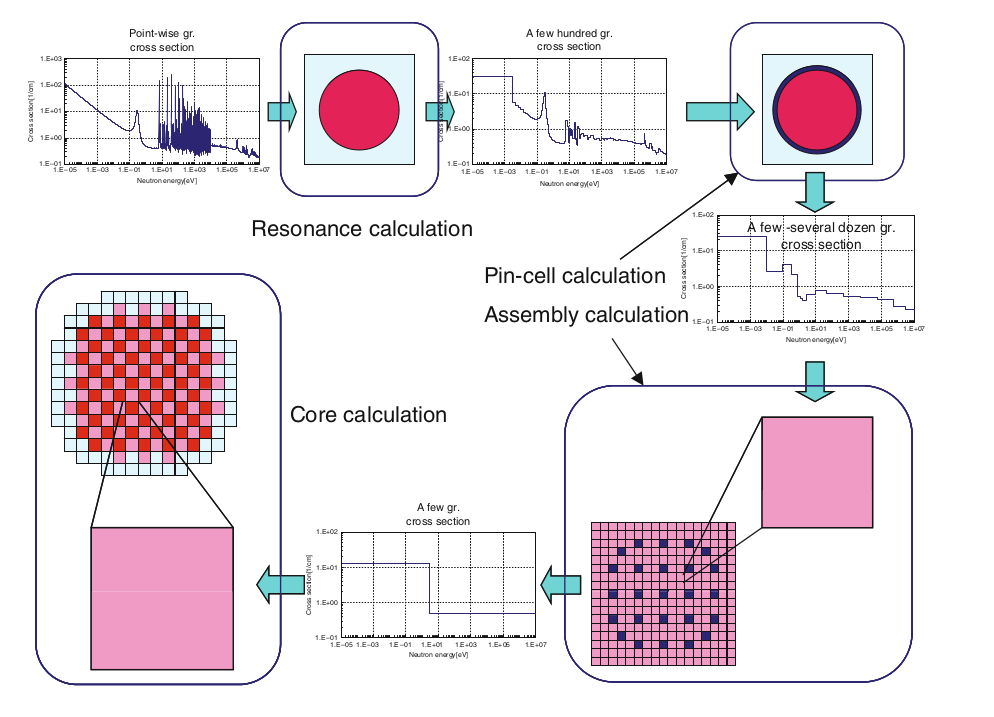
\includegraphics[width=0.70\linewidth]{generalCalculation.png}}
\blfootnote{Image credit: Cacuci, D. G. (Ed.). (2010). Handbook of Nuclear Engineering:  Springer Science \& Business Media. }
\end{frame}

\begin{frame}{Multigroup Neutron Transport Equation}
\begin{align}
\Omega \cdot \nabla \psi_g \left( r, \Omega \right) + \mathlarger{\sum}_{iso} N_{iso} \sigma_{t,iso,g} (r) \psi_g \left( r, \Omega \right) &= \mathlarger{\sum}_{g'=1}^G \mathlarger{\int}_{4\pi} \mathlarger{\sum}_{iso}  N_{iso} \sigma_{s,iso,g' \to g} \left( r, \Omega' \cdot \Omega \right) \psi_{g'} \left( r, \Omega' \right) d\Omega' \nonumber \\ 
&+ \frac{\chi_g (r)}{4\pi k} \mathlarger{\sum}  \mathlarger{\int}_{4\pi} \mathlarger{\sum}_{iso}  N_{iso} \nu \sigma_{f,iso,g'} (r) \psi_{g'} \left( r, \Omega' \right) d\Omega' 
\end{align}
\end{frame}

\begin{frame}{Multigroup Definitions}
\begin{subequations}
\begin{align}
\psi_g \left( r, \Omega \right) &= \int_{E_g}^{E_{g-1}} \psi \left( r, \Omega, E \right) dE \\
\sigma_{x,iso,g} \left( r, \Omega \right) &= \frac{ \mathlarger{\int}_{E_g}^{E_{g-1}} \sigma_{x,iso} \left( r, E \right) \psi \left( r, \Omega, E \right) dE}{ \mathlarger{\int}_{E_g}^{E_{g-1}} \psi \left( r, \Omega, E \right) dE} \\
\sigma_{s,iso,g' \to g} \left( r, \Omega' \cdot \Omega \right) &= \frac{\mathlarger{\int}_{E_g}^{E_{g-1}}\mathlarger{\int}_{E_g'}^{E_{g'-1}} \sigma_{s, iso} \left( r, \Omega' \cdot \Omega, E' \to E \right) \psi \left( r, \Omega, E' \right) dE' dE}{\mathlarger{\int}_{E_g'}^{E_{g'-1}} \psi \left( r, \Omega, E' \right) dE'} \\
\chi_g \left( r \right) &= \int_{E_g}^{E_{g-1}} \chi \left( r, E \right) dE
\end{align}
\end{subequations}
\end{frame}

%slide
\begin{frame}{Energy Self-Shielding}
  \centering
	\fcolorbox{fall}{white}{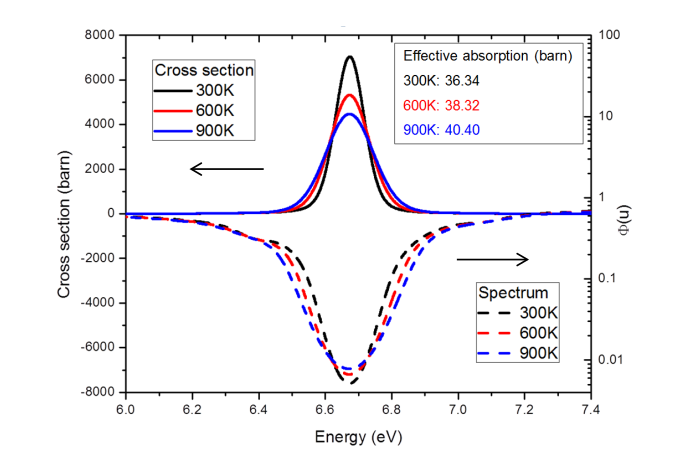
\includegraphics[width=0.70\linewidth]{energy2.png}}
\end{frame}

%slide
\begin{frame}{Energy Self-Shielding}
  \centering
	\fcolorbox{fall}{white}{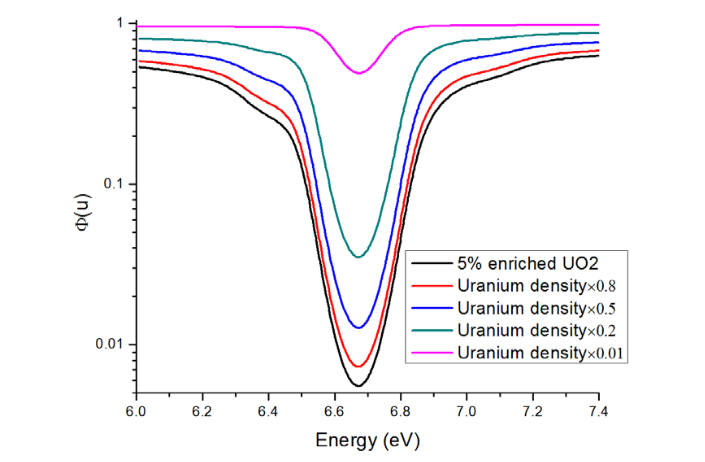
\includegraphics[width=0.70\linewidth]{energy1.png}}
\end{frame}

%slide
\begin{frame}{Spatial Self-Shielding}
  \centering
	\fcolorbox{fall}{white}{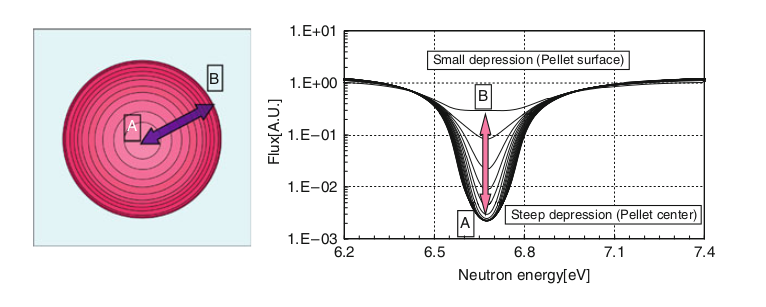
\includegraphics[width=0.80\linewidth]{spatial.png}}
\end{frame}

%slide
\begin{frame}{Self Shielding Calculation Approaches}
\begin{itemize}[<+->]
\item Direct solution of the \emph{slowing down calculation}
	\begin{itemize}[<+->]
	\item Fission source is neglected;
	\item Upscattering is neglected;
	\item Scattering source only considers isotropic s-wave elastic reactions.
	\end{itemize}
\item Precomputed integral tables
	\begin{itemize}[<+->]
	\item Bondarenko method
	\item Subgroup method
	\end{itemize}
\end{itemize}
\end{frame}

%slide
\begin{frame}{What to analyze and measure?}
\centering
\fcolorbox{fall}{white}{
\includegraphics[width=0.50\linewidth]{pin1.jpeg}}
\end{frame}

%slide
\begin{frame}{What to analyze and measure?}
\centering
\fcolorbox{fall}{white}{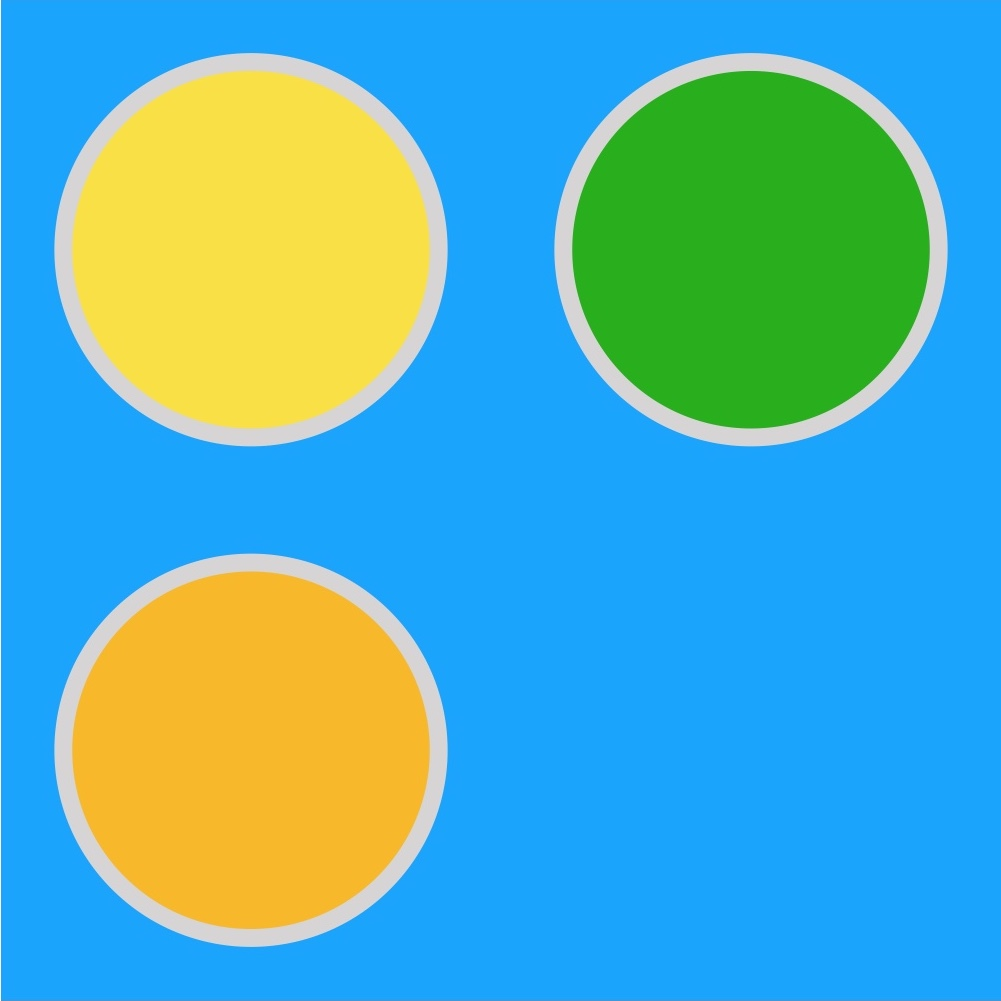
\includegraphics[width=0.50\linewidth]{pin2.jpeg}}
\end{frame}

%slide
\begin{frame}{What to analyze and measure?}
\centering
\fcolorbox{fall}{white}{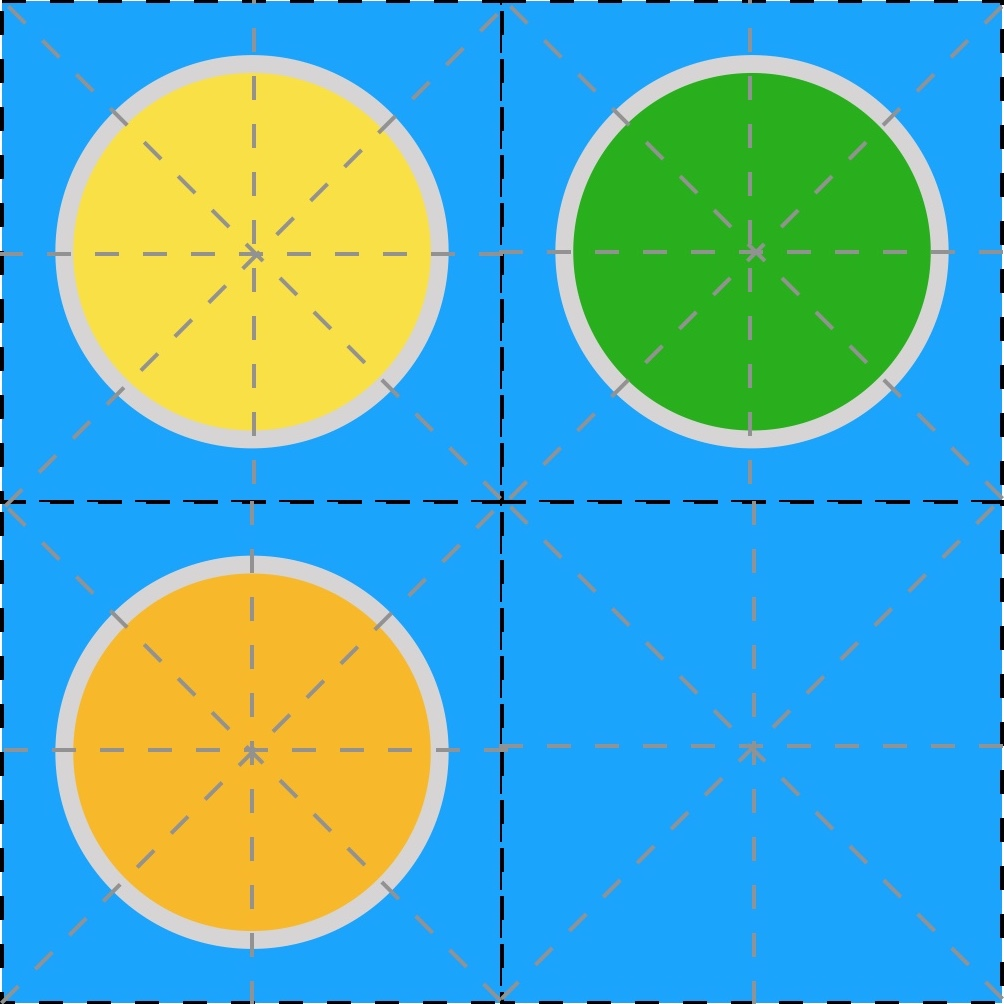
\includegraphics[width=0.50\linewidth]{pin3.jpeg}}
\end{frame}

%slide
\begin{frame}{Monte Carlo Options}
\begin{enumerate}[<+->]
\item MCNP
	\begin{itemize}[<+->]
	\item LANL, ~1950s (USA)
	\item Most established
	\end{itemize}
\item Serpent 
	\begin{itemize}[<+->]
	\item VTT, 2004 (Finland)
	\item Constant development and wide recognition 
	\end{itemize}
\item OpenMC
	\begin{itemize}[<+->]
	\item MIT, 2011 (USA)
	\item \emph{fully} Open Source
	\end{itemize}
\end{enumerate}
\end{frame}

%slide
\begin{frame}{OpenMC Demo}
\begin{itemize}
\item Cpp
\item Python and Cpp API
\item Jupyter-lab notebook 
\end{itemize}
\end{frame}

%slide
\begin{frame}{Other factors to consider}
\begin{itemize}
\item XS Generation
	\begin{itemize}[<+->]
	\item Deterministic vs Stochastic methodology
	\item Gemma bias
	\end{itemize}
\item Library energy structure
	\begin{itemize}[<+->]
	\item Application
	\item 51g MPACT LWR
	\item WIMS 69g and 172g (XMAS) LWR
	\item SHEM 281g
	\end{itemize}

\item Library generation with NJOY
\end{itemize}
\end{frame}

%slide
\begin{frame}
\centering
\Huge
Thanks! \\
Questions?
\end{frame}


\end{document}
